\begin{center}
   \Large{\textbf{Работа 1.2.4: Определение главных моментов инерции твердых тел с помощью крутильных колебаний}}
\end{center}
\section{Аннотация}
\textbf{Цель работы:}  измерить периоды крутильных колебаний рамки при
различных положениях закрепленного в ней тела, проверить теоретическую зависимость между периодами крутильных колебаний тела
относительно различных осей, определить моменты инерции относительно нескольких осей для каждого тела, по ним найти главные
моменты инерции тел и построить эллипсоид инерции.

\section{Теоретические сведения}
Инерционные свойства твердого тела при вращении определяет не
только величина его массы, но и ее пространственное распределение.
Последнее характеризует физическая величина, которая называется
тензором инерции. Геометрическим образом тензора инерции является эллипсоид,
уравнение которого в главных осях имеет вид: \begin{gather}
   I_x x^2 + I_y y^2 + I_z z^2 = 1
\end{gather}
Этот эллипсоид принято называть эллипсоидом инерции. Эллипсоид
инерции жестко связан с телом, для которого построен. Знание эллипсоида инерции
позволяет найти момент инерции тела относительно любой оси, проходящей через
центр эллипсоида. Для этого необходимо вдоль выбранной оси провести
радиус-вектор $ \vec{r} $ до пересечения с поверхностью эллипсоида. Длина $ r $  будет определять
момент инерции тела относительно этой оси: \begin{gather}
   I = \dfrac{1}{r^2}
\end{gather}
Главные оси тела часто можно определить из
его симметрии. Например, оси симметрии цилиндра или шара являются главными осями, так как
для всех осей, лежащих в плоскости перпендикулярной оси симметрии, моменты инерции одинаковые, и, следовательно, эллипсоид инерции обладает такой же симметрией, являясь эллипсоидом вращения относительно оси симметрии тела.
Крутильные колебания рамки с телом описываются уравнением \begin{gather}
   (I + I_p)\frac{d^2\phi}{dt^2} = - f \phi
\end{gather}
Здесь $ I $ и $ I_p $ -- это моменты инерции тела относительно оси вращения, $ \phi $ -- угол поворота рамки, $ f $ -- модуль кручения проволоки.
Период крутильных колебаний рамки с телом определяется формулой \begin{gather}
   T = 2\pi\sqrt{\frac{I + I_p}{ f}}
\end{gather}
Момент инерции относительно диагонали $ I_d $ выражается через главные моменты с помощью формулы: \begin{gather}
   I_d = I_x \frac{a^2}{x^2} + I_y\frac{b^2}{y^2} + I_z\frac{c^2}{z^2} \\
   (a^2 + b^2 + c^2)I_d = a^2I_x + b^2 I_y + c^2 I_z \\
   (a^2 + b^2 + c^2)T_d^2 = a^2T^2_x + b^2 T^2_y + c^2 T^2_z \label{firstcheck}
\end{gather}
Относительно остальных осей: \begin{gather}
   (b^2 + c^2)T^2_E = b^2 T_y^2 + c^2 T_z^2 \label{2check} \\
   (a^2 + c^2)T^2_P = a^2 T_x^2 + c^2 T_z^2 \label{3check}\\
   (b^2 + a^2)T^2_M = a^2 T_y^2 + b^2 T_z^2 \label{4check}
\end{gather}
\section{Методика измерений}
В данной работе используется устройство для получения крутильных колебаний, изображенное на рис.\ref{fig:scheme}. Рамка 1 жестко соединена
с проволокой 2, закрепленной вертикально в специальных зажимах
3, позволяющих сообщить начальное закручивание для возбуждения
крутильных колебаний вокруг вертикальной оси. В рамке с помощью
планки 4, гаек 5 и винта 6 закрепляется твердое тело 7. На теле имеются специальные выемки, позволяющие его закрепить так, чтобы ось
вращения проходила в теле под различными углами через центр масс.
 \begin{figure}[h]
   \centering
   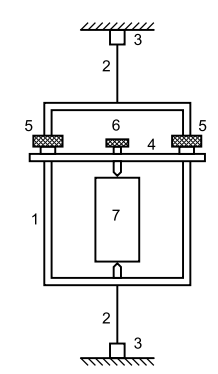
\includegraphics[width = 0.25\textwidth]{images/1.png}
   \caption{Схема установки}
   \label{fig:scheme}
\end{figure}

В работе будем проверять соотношения \eqref{firstcheck}, \eqref{2check}, \eqref{3check} и \eqref{4check}.
Для пустой рамки и всех тел при различных их положениях относительно оси колебаний определим периоды колебаний по времени 10-15
колебаний, повторяя каждое измерение не менее 3 раз. Штангенциркулем измерьте
геометрические размеры параллелепипеда. Вычислите главные моменты инерции. По
полученным ранее данным проверьте справедливость формул.
\section{Используемое оборудование}
\textbf{В работе используются:} установка для получения крутильных
колебаний (жесткая рамка, имеющая винты для закрепления в ней
твердых тел, подвешенная на натянутой вертикально проволоке), набор исследуемых твердых тел, секундомер.
\textbf{Погрешности:}\begin{enumerate}
   \item  Для секундомера $ \pm 0,5~c $
   \item Для линейки $ \pm 0,5\text{ мм } $
   \item Для транспортира $ \pm 0,5^\circ $
\end{enumerate}
\section{Результаты и обработка измерений}
\begin{table}[!h]
   \centering\caption{Пустая рамка и цилиндры}
   \begin{tabular}{|c|c|c|c|c|}
   \hline
       Периоды 10 измерений, с& Пустая рамка & Мал. Цил.,  z & Мал. Цил.,  x & Бол. Цил., z \\ \hline
       1 & 25,56 & 32,12 & 30,57 & 31,90 \\ \hline
       2 & 25,65&32,06 & 30,40 & 31,94 \\ \hline
       3 & 25,52&32,18 & 30,27 & 31,63 \\ \hline
       10T, секунд & 25,58& 32,12 & 30,41 & 31,82 \\ \hline
       T, секунд & 2,558 &3,212 & 3,041 & 3,182 \\ \hline
   \end{tabular}
\end{table}
\begin{table}[!h]
   \centering\caption{Цилиндры и главные оси куба}
   \begin{tabular}{|c|c|c|c|c|c|}
   \hline
       Периоды 10 измерений, с & Бол. Цилиндр, x & Два цилиндра & Куб, z  & Куб, x  & Куб, z  \\ \hline
       1 & 34,23 & 37,10 & 30,57  & 30,66  & 30,72  \\ \hline
       2 & 34,59 & 36,88 & 30,65  & 30,55  & 30,78  \\ \hline
       3 & 34,45 & 36,95 & 30,69  & 30,62  & 30,64  \\ \hline
       10T, секунд & 34,42 & 36,98 & 30,64  & 30,61  & 30,71  \\ \hline
       T, секунд & 3,442 & 3,698 & 3,064 & 3,061  & 3,071  \\ \hline
   \end{tabular}
\end{table}
\begin{table}[!h]
   \centering
   \caption{Куб: диагонали и другие}
   \begin{tabular}{|c|c|c|c|c|}
   \hline
       Периоды, с & Плоскостная диагональ  & Главная диагональ & Куб / 2 & Куб / 3  \\ \hline
       1 & 30,67 & 30,73 & 30,65 & 30,67  \\ \hline
       2 & 30,81 & 30,80 & 30,74 & 30,79  \\ \hline
       3 & 30,70 & 30,65 & 30,64 & 30,63  \\ \hline
       10T, секунд & 30,73 & 30,73 & 30,68 & 30,70  \\ \hline
       T, секунд & 3,073 & 3,073 & 3,068 & 3,070  \\ \hline
   \end{tabular}
\end{table}
\begin{table}[!h!]
   \centering
   \caption{Параллелепипед: главные}
   \begin{tabular}{|c|c|c|c|}
   \hline
       Периоды 10 измерений, с & T, z& T, x& T, y \\ \hline
       1 & 40,80 & 38,03 & 32,70  \\ \hline
       2 & 40,69 & 37,91 & 32,58  \\ \hline
       3 & 40,71 & ~ &   \\ \hline
       10T, секунд & 40,73 & 37,97 & 32,64  \\ \hline
       T, секунд & 4,073 & 3,797 & 3,264  \\ \hline
   \end{tabular}
\end{table}
\begin{table}[ht!]
   \centering
   \caption{Параллелепипед: диагонали}
   \begin{tabular}{|c|c|c|}
   \hline
       Периоды 10 измерений, с & T, плоскостная диагональ & T, главная  \\ \hline
       1 & 33,34 & 35,03  \\ \hline
       2 & 33,47 & 35,03  \\ \hline
       10T, секунд & 33,41 & 35,03  \\ \hline
       T, секунд & 3,341 & 3,50  \\ \hline
   \end{tabular}
\end{table}

\begin{table}[!h!]
   \centering
   \caption{Характеристики цилиндров}
   \begin{tabular}{|c|c|c|}
   \hline
       Характеристики & Мал. Цилиндр & Бол. Цилиндр \\ \hline
       d, мм & 87,6 & 87,8 \\ \hline
       h, мм & 49,4 & 97,5 \\ \hline
       m, г & 2263,6 & 4562,4 \\ \hline
   \end{tabular}
\end{table}


\begin{table}[!h]
   \centering
   \caption{Массы кубиков в граммах}
   \begin{tabular}{|c|c|}
   \hline
       2 & 1085,5  \\ \hline
       3 & 1090,5  \\ \hline
       6 & 1086,9  \\ \hline
   \end{tabular}
\end{table}
Длина ребра куба 6: $ a = 93,4 \text{ мм } $
\begin{table}[!ht]
   \centering
   \caption{Характеристика параллелепипеда}
   \begin{tabular}{|c|c|}
   \hline
       m, г & 1083,2 \\ \hline
       x, мм & 100,4 \\ \hline
       y, мм & 150,3 \\ \hline
       z, мм & 50,7 \\ \hline
   \end{tabular}
\end{table}

 \begin{table}[!ht]
   \caption{Главные моменты инерции}
   \centering
   \begin{tabular}{|c|c|c|c|}
   \hline
       Предмет & $ \frac{I + I_x}{f}, c^2 $ & $ \frac{I + I_y}{f}, c^2 $ & $ \frac{I + I_z}{f}, c^2 $ \\ \hline
       Пустая рамка & ~ & ~ &  0,166  \\ \hline
       Маленький цилиндр &  0,234  &  0,234  &  0,261  \\ \hline
       Большой цилиндр &  0,300  &  0,300  &  0,257  \\ \hline
       Два цилиндра & ~ & ~ &  0,346  \\ \hline
       Куб 6 &  0,237  &  0,239  &  0,238  \\ \hline
       Куб 2 & ~ & ~ &  0,238  \\ \hline
       Куб 3 & ~ & ~ &  0,239  \\ \hline
       Параллелепипед &  0,365  &  0,270  &  0,420 \\ \hline
   \end{tabular}
\end{table}
\newpage
\begin{table}[!ht]
   \centering
   \caption{Погрешности $T^2$}
   \begin{tabular}{|c|c|c|c|c|c|c|c|c|c|}
   \hline
       Пустая рамка & Мал. Цилиндр,  z & Мал. Цилиндр,  x & Бол. Цилиндр, z & Бол. Цилиндр, x \\ \hline
       0,256 & 0,321 & 0,304 & 0,318 & 0,344 \\ \hline
   \end{tabular}
\end{table}
\begin{table}[!ht]
   \centering
   \caption{Погрешности $T^2$}
   \begin{tabular}{|c|c|c|c|c|c|c|c|c|}
   \hline
       Два цилиндра & Куб, z & Куб, x & Куб, y & Куб, диагональ xz & Куб глав д & Куб / 2 & Куб / 3\\ \hline
       0,370 & 0,306 & 0,306 & 0,307 & 0,307 & 0,307 & 0,307 & 0,307  \\ \hline
   \end{tabular}
\end{table}
\begin{table}[!ht]
   \centering
   \caption{Погрешности $T^2$}
   \begin{tabular}{|l|l|l|l|l|}
   \hline
       Параллелепипед, z & Параллелепипед, x & Параллелепипед, y & Параллел.,пл. & Параллел., гл. \\ \hline
       0,407 & 0,380 & 0,326 & 0,334 & 0,350 \\ \hline
   \end{tabular}
\end{table}
Тогда у $ T^2 $ погрешность равна $ 2\Delta T$. Поскольку мерили по 10, то $ \Delta T = 0,05~c $, поэтому $ \epsilon_{T^2} = \epsilon_T $. \begin{gather}
   \Delta_{T_\text{ ср }} \approx 0,10~c^2 \\
   \frac{I + I_p}{f} = \frac{T^2}{4\pi^2}\, \implies \Delta\left(\frac{I + I_p}{f}\right) = \frac{\Delta T^2}{4\pi^2} \approx 3,1\%
\end{gather}
 

Построим сечение эллипсоидом инерции тела, для этого вычислим $ \dfrac{1}{\sqrt{T^2 - T_p^2}} $:
\begin{table}[!ht]
   \centering
   \caption{Расстояния}
   \begin{tabular}{|c|c|}
   \hline
      Тело & $ \dfrac{1}{\sqrt{T^2 - T_p^2}}, c^{-1} $ \\ \hline
       Маленький Цилиндр,  z & 0,27 \\ \hline
       Маленький Цилиндр,  x & 0,37 \\ \hline
       Большой Цилиндр, z & 0,28 \\ \hline
       Большой Цилиндр, x & 0,19 \\ \hline
       Куб, z & 0,35 \\ \hline
       Куб, x & 0,35 \\ \hline
       Куб, y & 0,34 \\ \hline
       Параллелепипед, z & 0,10 \\ \hline
       Параллелепипед, x & 0,13 \\ \hline
       Параллелепипед, y & 0,24 \\ \hline
   \end{tabular}
\end{table}
\begin{figure}[!h]
   \begin{minipage}[h]{0.49\linewidth}
   \center{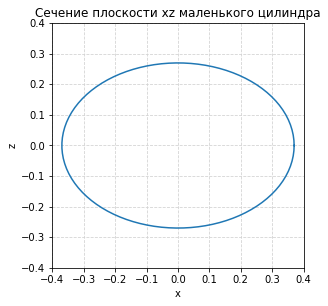
\includegraphics[width=0.9\linewidth]{images/2.png}}
   \end{minipage}
   \hfill
   \begin{minipage}[h]{0.49\linewidth}
   \center{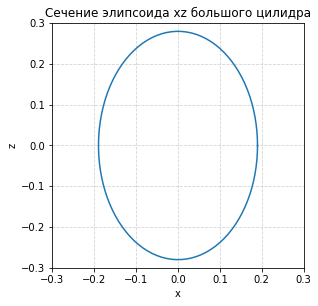
\includegraphics[width=0.9\linewidth]{images/3.png}}
   \end{minipage}
\end{figure}
\begin{figure}[!h]
   \begin{minipage}[h]{0.49\linewidth}
   \center{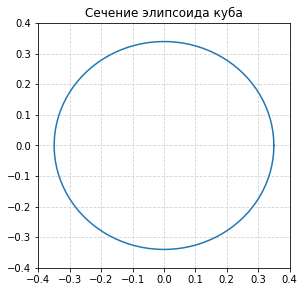
\includegraphics[width=0.9\linewidth]{images/4.png}}
   \end{minipage}
   \hfill
   \begin{minipage}[h]{0.49\linewidth}
   \center{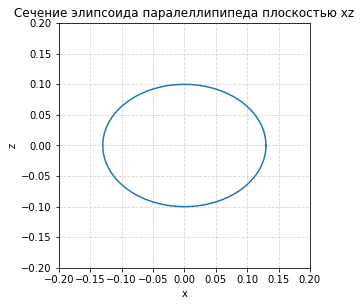
\includegraphics[width=0.9\linewidth]{images/5.png}}
   \end{minipage}
\end{figure}
\begin{figure}[!h]
   \begin{minipage}[h]{0.49\linewidth}
   \center{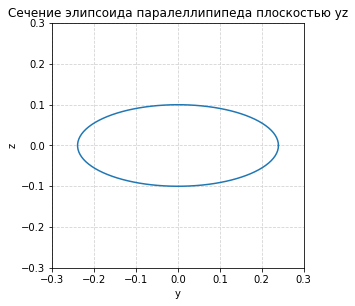
\includegraphics[width=0.9\linewidth]{images/6.png}}
   \end{minipage}
   \hfill
   \begin{minipage}[h]{0.49\linewidth}
   \center{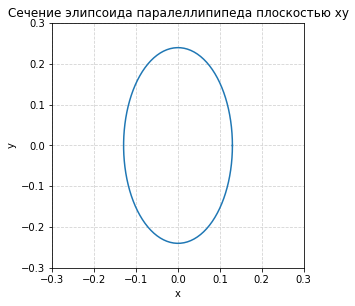
\includegraphics[width=0.9\linewidth]{images/7.png}}
   \end{minipage}
\end{figure}
\newpage
\section{Обсуждение результатов} 
Проверим верность формул \eqref{firstcheck}, \eqref{2check}, \eqref{3check} и \eqref{4check}:

Для куба: \begin{gather}
   T_ \text{ плоскостная диагональ }^2(a^2 + a^2) \overset{?}{=} a^2T_y^2 + b^2T_z^2 \\
   3,073^2 \cdot 2 - (3,064^2 + 3,071^2) = 0,068~\text{ м }c^2 < 0,1~\text{м}c^2
\end{gather} \begin{gather}
   T_\text{ главная диагональ }^2 3a^2 \overset{?}{=} a^2 T_x^2 + a^2 T_y^2 + a^2 T_z^2 \\
   3 \cdot 3,073^2 - (3,061^2 + 3,064^2 + 3,071^2) = 0,068~\text{ м }c^2 < 0,1~\text{м}c^2
\end{gather}
Для параллелепипеда: \begin{gather}
   T_ \text{ плоскостная диагональ }^2(a^2 + b^2) \overset{?}{=} a^2T_y^2 + b^2T_z^2 \\
   3,341^2(0,1503^2 + 0,0507^2) - (0,1503^2 \cdot 3,797^2 + 0,0507^2 \cdot 3,264^2) = - 0,073 \text{ м }c^2 >-0,1 \text{ м }c^2
\end{gather} \[
   T_\text{ главная диагональ }^2 (a^2 + b^2 + c^2) \overset{?}{=} a^2 T_x^2 + b^2 T_y^2 + c^2 T_z^2 \]
   \begin{multline}
   (0,1503^2 + 0,507^2 + 0,1004^2) \cdot 3,50^2 - (0,1503^2 \cdot 4,073^2 + 0,0507^2 \cdot 3,264^2 +\\+ 0,1004^2 \cdot 3,797^2) = 0,053 \text{ м }c^2 < 0,1 \text{ м }c^2
\end{multline}
Значит формулы верны в пределах нашей погрешности.
Для соосных цилиндров должно выполняться: \begin{gather}
   \frac{I_\text{ маленький z}}{m}  = \frac{I_\text{ большой z }}{M}  = \frac{I_\text{ двух z }}{m + M}
\end{gather}
Используя теоретическую формулу для $ I = \frac{1}{6}m a^2 $ найдём $ f $: \begin{gather}
   \begin{cases} 
      I_p = 0,166f \\
      I_t = \dfrac{1}{6} \cdot 1,0869 \cdot 0,0934^2 = 1,58 \cdot 10^{ - 3}~\text{ кг } \cdot \text{ м }^2 \\
      I_t = 0,238f - I_p
   \end{cases} \implies 1,58 \cdot 10^{ - 3} = 0,072f \\
   f = 0,0219~\frac{\text{ кг } \cdot \text{ м }^2}{\text{ с }^2}
\end{gather}
Погрешность $ f $: \begin{gather}
   \epsilon_f = \frac{5 \cdot 10^{ - 3}}{0,072} = 7 \% \implies \Delta f = 1,5 \cdot 10^{ - 3}~\frac{\text{ кг } \cdot \text{ м }^2}{\text{ с }^2}
\end{gather}
\begin{table}[!ht]
   \centering
   \caption{Главные моменты инерции}
   \begin{tabular}{|c|c|c|c|}
   \hline
       Предмет & I, x, $\text{ г } \cdot \text{ м }^2$ & I, y, $\text{ г } \cdot \text{ м }^2$ & I, z, $\text{ г } \cdot \text{ м }^2$ \\ \hline
       Пустая рамка & ~ & ~ &  3,6  \\ \hline
       Маленький цилиндр &  1,5  &  1,5  &  2,1  \\ \hline
       Большой цилиндр &  2,9  &  2,9  &  2,0  \\ \hline
       Два цилиндра & ~ & ~ &  4,0  \\ \hline
       Куб 6 &  1,6  &  1,6  &  1,6  \\ \hline
       Куб 2 & ~ & ~ &  1,6  \\ \hline
       Куб 3 & ~ & ~ &  1,6  \\ \hline
       Параллелепипед &  4,4  &  2,3  &  5,6 \\ \hline
   \end{tabular}
\end{table}
Погрешность вычисленного $ I $: \begin{gather}
   \Delta I \leq 0,61 \text{ г } \cdot \text{ м }^2
\end{gather}
Тогда данное значение $ f $ не соответствует значению для маленького цилиндра. Возможно данное расхождение произошло из-за того, что 
не была учтена случайная погрешность измерений или периоды для какого-то из цилиндров измерялись при углах, при которых уже нельзя пользоваться гармоническими законами для
вычисления $ \frac{I + I_p}{f}  $. Кроме того, возможно, что во время работы $ f $ поменялось.
\section{Вывод}
Удалось измерить периоды крутильных колебаний рамки при различных положениях закреплённого в ней тела, подтвердили верность теоретическую зависимость между периодами крутильных колебаний тела относительно различных осей, нашли главные моменты инерции тел и построили дл них эллипсоиды инерции. Однако погрешности данных измерений оказались очень большими.

